%
%	Protocol template 
%	version 1.1
%	16.10.2014
%
\newcommand{\TITLE}{
% + + TITLE + +
Dedicated Sensor Array
% - -  TITLE - -
}
\newcommand{\VERSION}{
% + + TITLE + +
2
% - -  TITLE - -
}

% DO NOT CHANGE FROM HERE
%
%	Protocol configuration 
%	version 1.4
%	22.02.2016
%
\documentclass[a4paper,12pt]{article}
\usepackage[english]{babel}
\usepackage[pdftex]{graphicx}
\usepackage{pdfpages}
\usepackage{textcomp}
\usepackage{pdflscape}
\usepackage{array}
\usepackage{placeins}
\usepackage{floatflt}
\usepackage{float}
\usepackage{caption}
\usepackage{subcaption}
\usepackage{wrapfig}
\usepackage{pgfplots}
\usepackage{ulem}
\usepackage[absolute]{textpos}
\usepackage{ragged2e}
\usepackage{epstopdf}
%paper
\usepackage{a4wide}
\usepackage{scrpage2}
\usepackage[onehalfspacing]{setspace}
\usepackage{lastpage}
\pagenumbering{arabic}
\pagestyle{scrheadings}
%font
\usepackage[utf8]{inputenc}
\usepackage[T1]{fontenc}
\usepackage[babel,german=swiss]{csquotes}
%markup
\usepackage{amsmath}
\usepackage{extarrows}
\usepackage{amssymb}
\usepackage[ampersand]{easylist}
\usepackage[version=3]{mhchem}
\usepackage{chemfig}
\usepackage{titlesec}
\usepackage{multirow}
\usepackage{xifthen}
\newcolumntype{M}[1]{>{\centering\arraybackslash}m{#1}}
\newcolumntype{N}{@{}m{0pt}@{}}
%Roman numerals
\newcommand{\RM}[1]{\MakeUppercase{\romannumeral #1}}
%Substance numbering
\newcommand{\NB}[1]{(\textbf{#1})}
%NMR-printing
\newcommand{\NMR}[2]{\({}^{#1}\text{#2-NMR}\)}
%Print Et2O
\newcommand{\Ether}[0]{\(\text{Et}_{2}\text{O}\)}
%Symbol with circle
\newcommand\kreis[1]{\ensuremath{\mathbin{\settowidth{\dimen7}{\mbox{$ \bigcirc$}}\makebox[0pt][l]{$\bigcirc$}\makebox[\dimen7]{#1}}}}
%Format substance in reaction - Usage: \Sub[Number(optional)]{Formular(math-env enabled)} -> \Sub{[1]}{H_2O} -- \Sub{H_20}
\newcommand\Sub[2][]{
	\ifthenelse{\isempty{#1}}
	%true
	{$#2$}
	%false
	{$\underset{\NB{#1}}{#2}$}
}
%Reaction arrow [#1=Temp] {#2=chemicals} {#3=time}
\newcommand\RA[4][]{
	\ifthenelse{\isempty{#1}}
	{\ifthenelse{\isempty{#4}}
		{$\xrightarrow[\textsf{#3}]{\textsf{,~#2~}}$ }
		{$\xrightarrow[\textsf{#3, #4}]{\textsf{~#2~}}$ }}	
	{\ifthenelse{\isempty{#4}}
		{$\xrightarrow[\begin{subarray}{c}\textsf{#3,} \\ \textsf{#1{}}^{\circ}\textsf{C}\end{subarray}]{\textsf{#2}}$}
		{$\xrightarrow[\begin{subarray}{c}\textsf{#3,} \\ \textsf{#1{}}^{\circ}\textsf{C},~\textsf{#4}\end{subarray}]{\textsf{#2}}$}}
}
\newcommand{\HRule}{\rule{\linewidth}{0.5mm}}
\newcommand{\TEMP}[1]{\ensuremath{\text{#1}^{\circ}\text{C}}}
\newcommand{\newtoday}{\the\day/\the\month/\the\year}
\newcommand{\water}{$\textrm{H}_{2}\textrm{O}$}
\newcommand{\waterSF}{\textsf{H}_{2}\textsf{O}}

%Lineheight
\renewcommand{\arraystretch}{1.5} 

\pagestyle{scrheadings}
\ihead{\TITLE}
\ohead{Marc Schäfer \& Max Hackinger}
\setfootsepline{0.5pt}
\setheadsepline{0.5pt}
\pagenumbering{arabic}
\ifoot{\newtoday}
\ofoot{\pagemark}
\begin{document}
%
%	Protocol titlepage template 
%	version 2 - ic practical course
%	15.10.2014
%
\begin{titlepage}
	\begin{center}
		% + + + + + TITLE: + + + + + 
		{\Large \bfseries Dedicated Sensor Array }
		
		\vspace{3cm}
		
		\begin{center}
			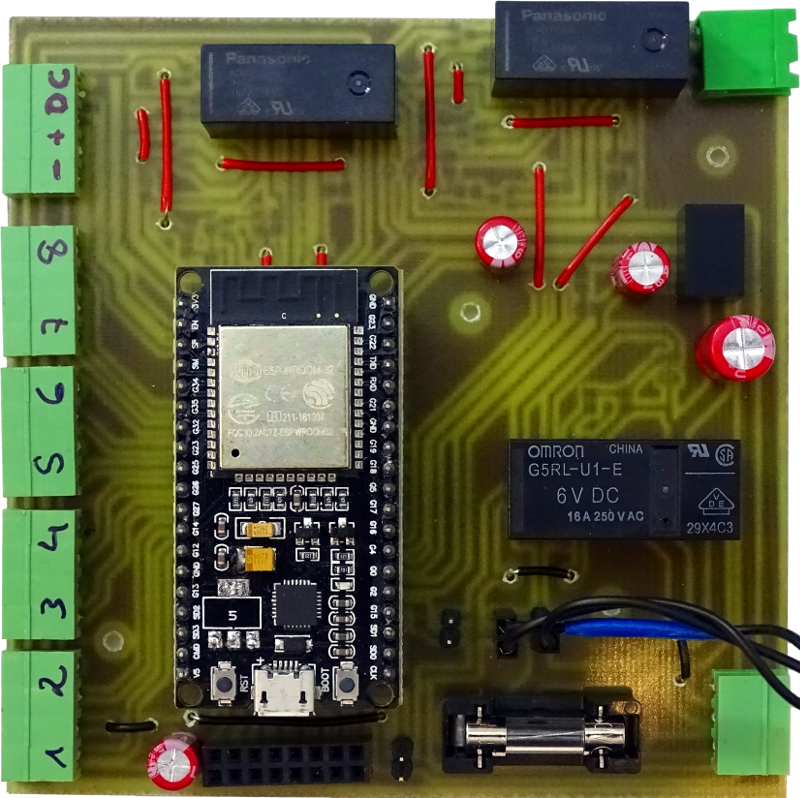
\includegraphics[width=0.5\linewidth]{../../pictures/sensorstation/small/DSC00289.png}
		\end{center}

		%
		\vfill
		
		
		% Date
		{\normalsize \newtoday } 
		
		% Author
		{\normalsize Max Hackinger \& Marc Schäfer}
		
		
		
	\end{center}
	%Language label
	\noindent
	\begin{flushleft} 
		%\textbf {English}
	\end{flushleft}
\end{titlepage}
% DO NOT CHANGE UNTIL HERE



\section{Introduction}
\justify

The Dedicated Sensor Array is in essence a system for measuring and collecting environmental data. The implementation is generic so the System can work with a variety of different sensor types and measure a large spectrum of environmental parameters. 


The System is composed of two parts, one central server and several dedicated sensor stations. The sensor stations are battery powered. It measures environmental parameters, evaluates the raw data and sends the values to the server over WiFi. The server receives, collects and makes the data accessible for additional applications. \\

The technical requirements for the server are a JVM and WiFi connectivity. The WiFi connectivity can either be a direct Hotspot created by the system running the JVM or the system can be part of a network with a WiFi bridge. The sensor station requires an ESP-WROOM-32 Module with an Espressif ESP32 MCU. \\

The sensor station has a low power design to offer a long runtime. They provide several, different ADC for the measurements, a potential free relay for triggering external events and a voltage supervisor to protect the battery against deep discharge. Furthermore, the power supply of the sensor station is extendable by a solar charging module.

For the moment there are three environmental parameters that are measurable: temperature, light intensity and magnetic field strength. For monitoring of the runtime the battery voltage can also be measured.

The server can handle multiple connections from several sensor stations. It combines and stores all sensor data received from every sensor station in a database table.\\


\section{Execution \& Technical Details}
The two parts, the server and the sensor station, were respectively assigned to one team member. The server was assigned to Max, the sensor station to Marc. Initially, the general framework was determined and interfaces were defined. Subsequently, the two parts were independently developed and successively aligned. This was necessary because of the completely new development environment regarding the ESP32 and the therefore unknown possibilities and obstacles.\\

The server is written in Java and uses the SQL database Apache Derby.
At first startup the database is automatically configured. It listens for TCP/IP connections on a configurable port. A JSON based protocol is used for communication between server and sensor station. The server waits for a JSON frame from the sensor station, processes the frame and responds in turn with a JSON frame, containing an acknowledgement and/or commands for the sensor station.\\

For the sensor station, a custom PCB was designed and made to connect the sensors and I${}^{2}$C bus. Additionally, the low dropout regulator (LDO) of the ESP-WROOM-32 dev board was replaced by a high-efficiency DC switching regulator. The sensors and the I${}^{2}$C bus can be fully turned off to save energy while not acquiring analog signals. The firmware for the ESP32 is written in C++.
The sensor station uses different run modes. In the normal run mode, the sensor station measures data, evaluates and stores it to the flash memory. Subsequently, it enters a lower run mode called deep sleep. In this mode, the sensor station uses just a fraction of the energy used in the normal run mode and can wait for a special event or for a specific time to wake up and enters the normal run mode again. After a defined amount of measuring cycles, the sensor station enters the communication mode and turns on WiFi. It connects to the server, sends all the collected data, waits for a response and enters the normal mode again. Received commands get processed and if necessary, the sensor station enters the communication mode again. Otherwise, the sensor station begins a new measuring cycle.
\begin{table}[htbp]
	\begin{center}
		\begin{tabular}{|l|c|c|c|}
			\hline 
			Mode: & Deep Sleep & Normal Operation & Communication \\ 
			\hline 
			Power: & 1-5 mA & 15-20 mA & 50-100 mA \\ 
			\hline 
		\end{tabular} 
	\end{center}
	\caption{Power consumption in different modes}
\end{table}\\

\newpage
\section{Downsizing}
The scope of our project needed to be reduced somewhat as dejan had to leave the group because of private reasons.
It was originally planned to create a GUI application that would represent the data that the Sensor Station sent the Server, but this proved to be too challenging for just the two of us.
The timing was especially unfortunate, because this happened midway through development, when they basics were defined but the details still had to be implemented and it therefore was too late to change the distribution of the tasks to compensate for the loss.
This lead to the project becoming a Dedicated Sensor Array with a flexible server, instead of a Weather Station with a touch screen to control the sensors and visualize the data.

\section{Conclusion}
On the microcontroller side, we discovered a little later then we would have liked that the NodeMCU Firmware that we were planning to use, was simply to resource intensive and buggy for our needs. This was not as big a problem as it could have been through, because we used the original Espressif ESP-IDF in combination with a Arduino plugin.

Another surprises was that the built in ADC (Analog to Digital Converter) on the ESP32 was insufficiently sensitive for our use case because of the unusual low input impedance. Thankfully there was an external ADC available which fulfilled the requirements.

Communication in the group worked well, even though we mostly meet remotely over Skype. However the project could have probably profited from a more regular frequency of meetings, for example twice a week. This might have made it clearer earlier on in the project that one of our members was overwhelmed and needed more support.
\newpage
\section{Pictures}
~
\begin{figure}[H]
	\begin{subfigure}[c]{\linewidth}
		\centering
		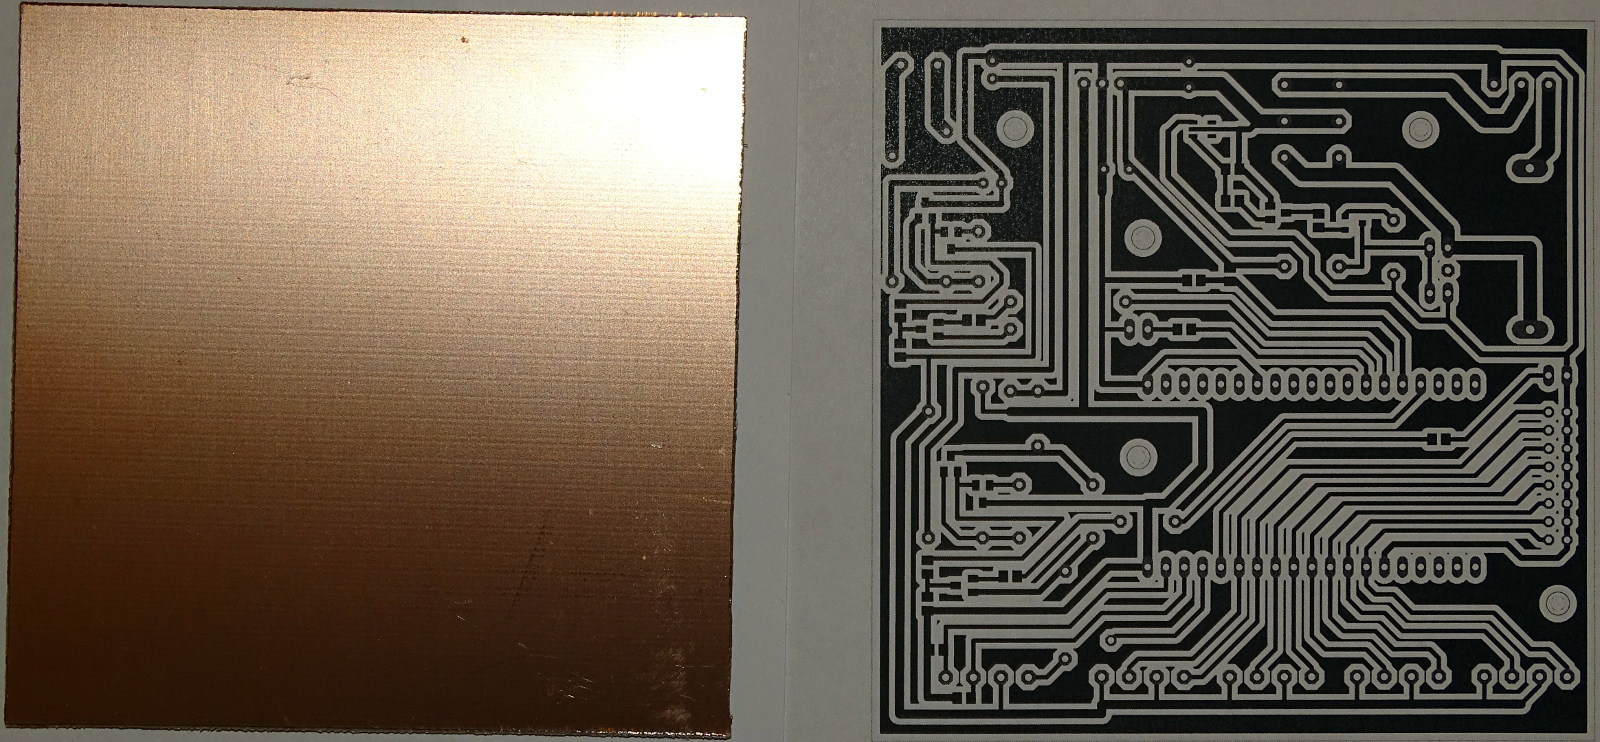
\includegraphics[width=\linewidth]{../../pictures/sensorstation/small/DSC00220.JPG}
		\subcaption{Raw board (left) and printed circuit layout (left)}		
	\end{subfigure}
	\begin{subfigure}[c]{0.5\linewidth}
		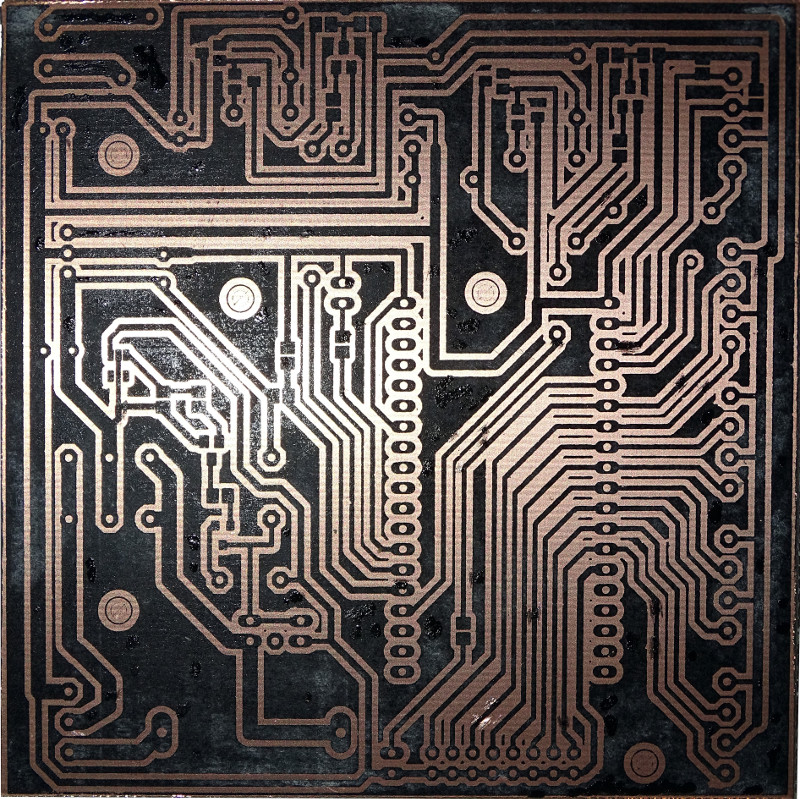
\includegraphics[width=\linewidth]{../../pictures/sensorstation/small/DSC00231.JPG}	
		\subcaption{Layout transferred to the board}		
	\end{subfigure}
	\begin{subfigure}[c]{0.5\linewidth}		
		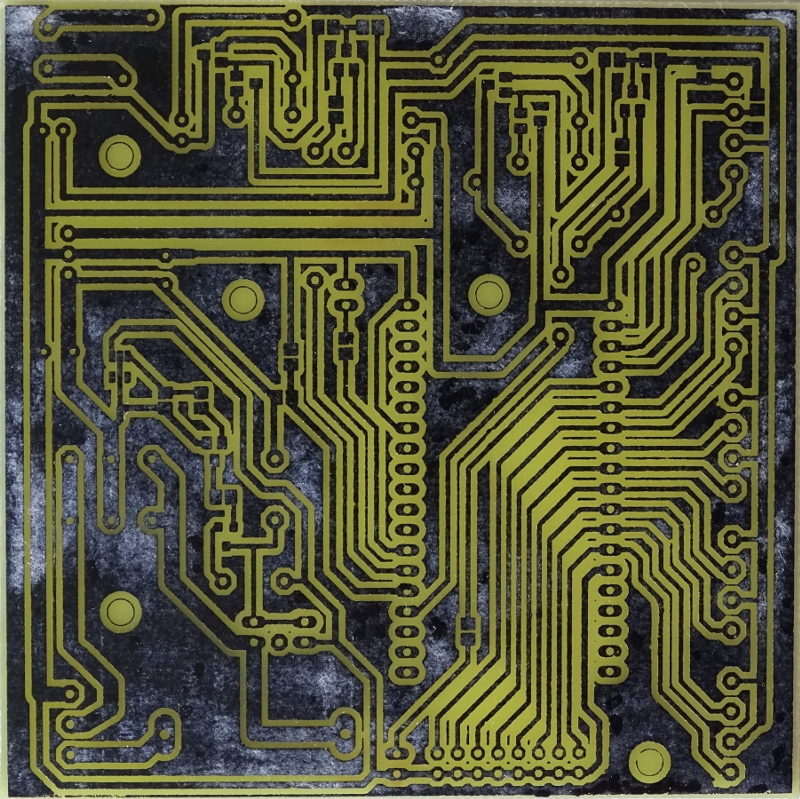
\includegraphics[width=\linewidth]{../../pictures/sensorstation/small/DSC00236.JPG}		
		\subcaption{Circuits etched into the board}
	\end{subfigure}
\end{figure}
\begin{figure}[H]
	\begin{subfigure}[c]{0.5\linewidth}	
		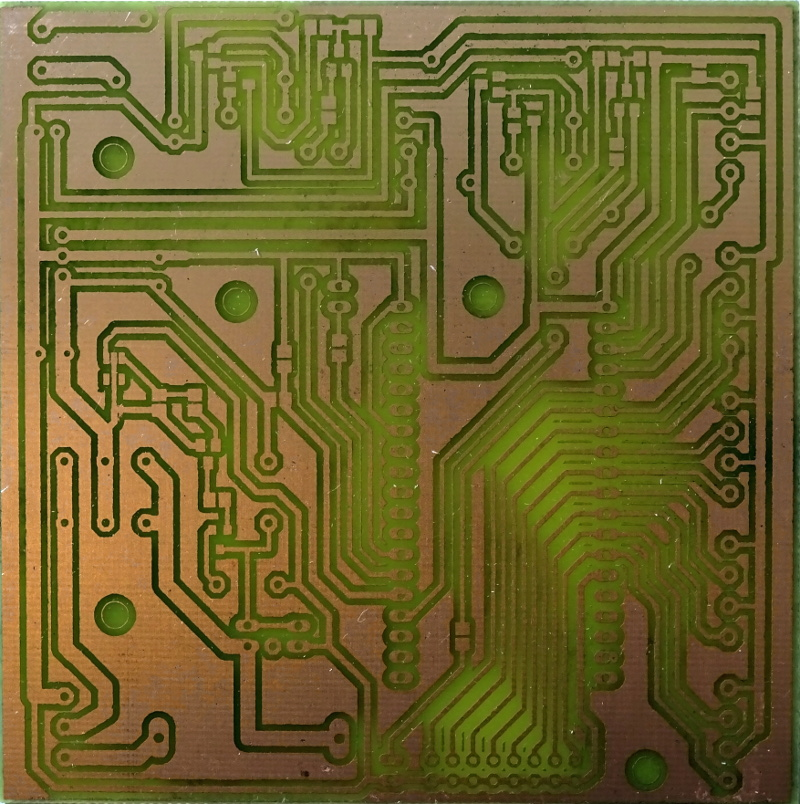
\includegraphics[width=\linewidth]{../../pictures/sensorstation/small/DSC00240.JPG}	
		\subcaption{PCB cleaned}
	\end{subfigure}
	\begin{subfigure}[c]{0.5\linewidth}	
		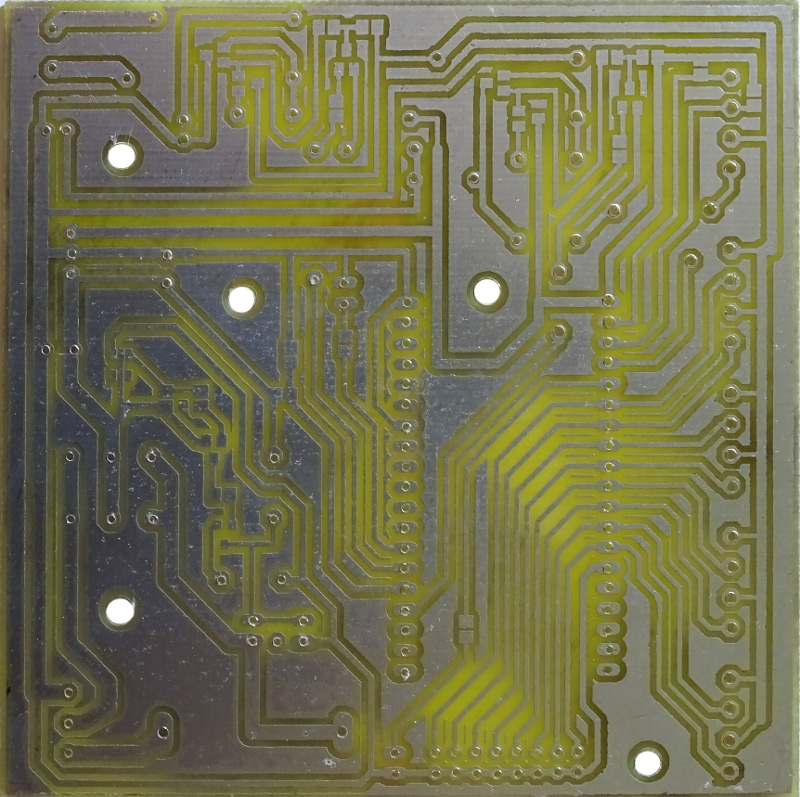
\includegraphics[width=\linewidth]{../../pictures/sensorstation/small/DSC00249.JPG}	
		\subcaption{Plated with tin}
	\end{subfigure}
	\begin{subfigure}[c]{0.5\linewidth}
		\centering
		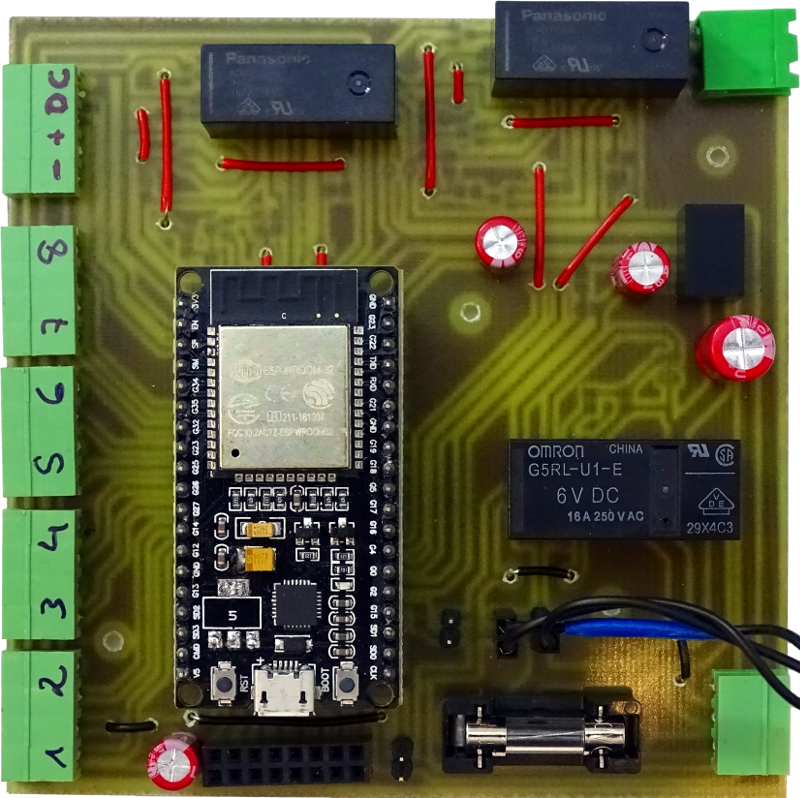
\includegraphics[width=\linewidth]{../../pictures/sensorstation/small/DSC00289.png}	
		\subcaption{Assembled PCB (top)}
	\end{subfigure}
	\begin{subfigure}[c]{0.5\linewidth}	
		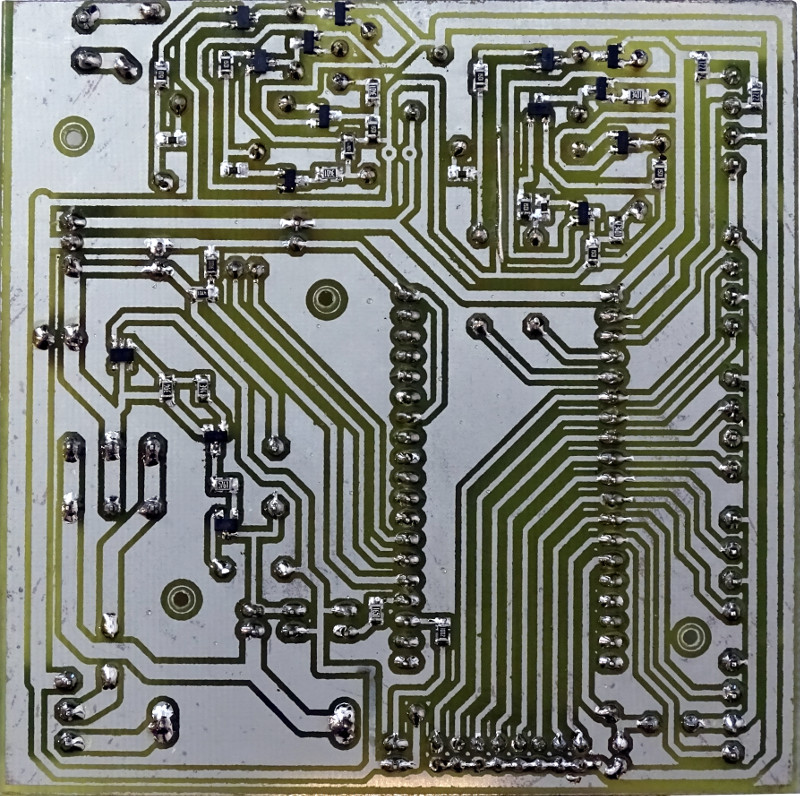
\includegraphics[width=\linewidth]{../../pictures/sensorstation/small/DSC00290.JPG}		
		\subcaption{Assembled PCB (bottom)}
	\end{subfigure}
\end{figure}
\newpage
\begin{thebibliography}{999}
	%\bibitem{litYield} J. P. Canal, T. R. Ramnial, L. D. Langlois, C. D. Abernethy, J. A. C. Clyburne, \textit{Lab Documentation: A Three Step Laboratory Sequence to Prepare a Carbene Complex of Silver(I) Chloride},
%	\bibitem{yield} L. Bannwart, \textit{Hausversuch Mayour Group - Step 2: Sonogashira Reaction of Höger-Acetylene with 1-Bromo-3-iodobenzene}, \textbf{2016}.
%	
%	\bibitem{complex1} UCDavis, \emph{Coordination Compounds}, http://chemwiki.ucdavis.edu/Core/\\Inorganic\_Chemistry/Coordination\_Chemistry/Coordination\_Compounds, 23.02.2016.
%	
%	\bibitem{complex2} UCDavis, \emph{Coordination Numbers and Geometry}, http://chemwiki.ucdavis.edu/Core/\\Inorganic\_Chemistry/Coordination\_Chemistry/Basics\_of\_Coordination\_Chemistry/\\Coordination\_Numbers\_and\_Geometry, 23.02.2016.
%	
%	
%
%\bibitem{harrowfield} J. MacB. Harrowfield,  G. A. Lawrance, A. M. Sargeson, \emph{Facile Synthesis of a Macrobicylic Hexaamine Cobalt(III) Complex Based on Tris(Ethylenediamine)Cobalt(III)},  Journal of Chemical Education, \textbf{1985}, vol. 62, \# 9, p. 804 - 806.
%
%
%\bibitem{clathrochelate} Y. Z. Voloshin,  N. A.a Kostromina, R. Krämer, "Clathrochelates: synthesis, structure, and properties" Elsevier, Amsterdam, 2002.
%
%\bibitem{peroxide} J. G. Carriazo,  E. A. Montoya-González, M. N. Vanoy-Villamil, \emph{Preparation and immobilization of diNOsarcobalt(III) complex in zeolite y for the catalyzed production of hydrogen peroxide}, Química Nova, \textbf{2013}, vol. 36, \# 9, pp. 1318-1322.
%
%\bibitem{synth1} R. A. Krause,  E. A. Megargle, \emph{Student Synthesis of Tris(ehtylenediamine)cobalt(\RM{3}) chloride}, Journal of Chemical Education, \textbf{1976}, vol. 53, p. 667.
%
%\bibitem{disc_synth1_1} R. A. Krause,  \emph{Why Green? More Chemistry in the Students Synthesis of Tris(ehtylenediamine)cobalt(\RM{3}) Chloride}, Journal of Chemical Education, \textbf{1978}, vol. 55, p. 453.
%
\bibitem{esp_idf} Espressif, ESP IDF, https://github.com/espressif/esp-idf.git
\bibitem{esp_idf_api} Espressif, ESP IDF API, https://esp-idf.readthedocs.io/en/latest/index.html
\bibitem{esp_toolchain} Espressif, Xtensa Toolchain, \newline https://www.espressif.com/en/products/hardware/esp32/resources
\bibitem{arduino}Espressif, ESP Arduino ESP32, https://github.com/espressif/arduino-esp32.git
\bibitem{mkfss} iggr, MKFSS, https://github.com/igrr/mkspiffs.git
\bibitem{json} bblanchon, Arduino JSON, https://github.com/bblanchon/ArduinoJson.git
\bibitem{ads1115} Adafruit, Adafruit ADS1X15, https://github.com/adafruit/Adafruit\_ADS1X15.git
\bibitem{derby} Apachce, Derby, https://db.apache.org/derby/
\bibitem{gson} Google, gson, https://github.com/google/gson


% TODO: JACS ref - OK
% JACS 2009 VOL 131 P. 14761-14767
%
%\bibitem{templatereactions} T. J. Marks, D. R. Stojakovic, \emph{Large metal ion-centered template reactions. Chemical and spectral studies of the "superphthalocyanine" dioxocyclopentakis(1-iminoisoindolinato)uranium(VI) and its derivatives}, J. Am. Chem. Soc., \textbf{1978}, vol. 100,  \# 6, p. 1695–1705.
\end{thebibliography}

%\includepdf[landscape=true,pages=-]{../Spectra/Expt4/4_2.pdf}

\end{document}